% Options for packages loaded elsewhere
\PassOptionsToPackage{unicode}{hyperref}
\PassOptionsToPackage{hyphens}{url}
%
\documentclass[
]{article}
\usepackage{lmodern}
\usepackage{amssymb,amsmath}
\usepackage{ifxetex,ifluatex}
\ifnum 0\ifxetex 1\fi\ifluatex 1\fi=0 % if pdftex
  \usepackage[T1]{fontenc}
  \usepackage[utf8]{inputenc}
  \usepackage{textcomp} % provide euro and other symbols
\else % if luatex or xetex
  \usepackage{unicode-math}
  \defaultfontfeatures{Scale=MatchLowercase}
  \defaultfontfeatures[\rmfamily]{Ligatures=TeX,Scale=1}
\fi
% Use upquote if available, for straight quotes in verbatim environments
\IfFileExists{upquote.sty}{\usepackage{upquote}}{}
\IfFileExists{microtype.sty}{% use microtype if available
  \usepackage[]{microtype}
  \UseMicrotypeSet[protrusion]{basicmath} % disable protrusion for tt fonts
}{}
\makeatletter
\@ifundefined{KOMAClassName}{% if non-KOMA class
  \IfFileExists{parskip.sty}{%
    \usepackage{parskip}
  }{% else
    \setlength{\parindent}{0pt}
    \setlength{\parskip}{6pt plus 2pt minus 1pt}}
}{% if KOMA class
  \KOMAoptions{parskip=half}}
\makeatother
\usepackage{xcolor}
\IfFileExists{xurl.sty}{\usepackage{xurl}}{} % add URL line breaks if available
\IfFileExists{bookmark.sty}{\usepackage{bookmark}}{\usepackage{hyperref}}
\hypersetup{
  pdftitle={Multi level model Analysis of Experiment 7},
  pdfauthor={Mrudula \& Carina},
  hidelinks,
  pdfcreator={LaTeX via pandoc}}
\urlstyle{same} % disable monospaced font for URLs
\usepackage[margin=1in]{geometry}
\usepackage{color}
\usepackage{fancyvrb}
\newcommand{\VerbBar}{|}
\newcommand{\VERB}{\Verb[commandchars=\\\{\}]}
\DefineVerbatimEnvironment{Highlighting}{Verbatim}{commandchars=\\\{\}}
% Add ',fontsize=\small' for more characters per line
\usepackage{framed}
\definecolor{shadecolor}{RGB}{248,248,248}
\newenvironment{Shaded}{\begin{snugshade}}{\end{snugshade}}
\newcommand{\AlertTok}[1]{\textcolor[rgb]{0.94,0.16,0.16}{#1}}
\newcommand{\AnnotationTok}[1]{\textcolor[rgb]{0.56,0.35,0.01}{\textbf{\textit{#1}}}}
\newcommand{\AttributeTok}[1]{\textcolor[rgb]{0.77,0.63,0.00}{#1}}
\newcommand{\BaseNTok}[1]{\textcolor[rgb]{0.00,0.00,0.81}{#1}}
\newcommand{\BuiltInTok}[1]{#1}
\newcommand{\CharTok}[1]{\textcolor[rgb]{0.31,0.60,0.02}{#1}}
\newcommand{\CommentTok}[1]{\textcolor[rgb]{0.56,0.35,0.01}{\textit{#1}}}
\newcommand{\CommentVarTok}[1]{\textcolor[rgb]{0.56,0.35,0.01}{\textbf{\textit{#1}}}}
\newcommand{\ConstantTok}[1]{\textcolor[rgb]{0.00,0.00,0.00}{#1}}
\newcommand{\ControlFlowTok}[1]{\textcolor[rgb]{0.13,0.29,0.53}{\textbf{#1}}}
\newcommand{\DataTypeTok}[1]{\textcolor[rgb]{0.13,0.29,0.53}{#1}}
\newcommand{\DecValTok}[1]{\textcolor[rgb]{0.00,0.00,0.81}{#1}}
\newcommand{\DocumentationTok}[1]{\textcolor[rgb]{0.56,0.35,0.01}{\textbf{\textit{#1}}}}
\newcommand{\ErrorTok}[1]{\textcolor[rgb]{0.64,0.00,0.00}{\textbf{#1}}}
\newcommand{\ExtensionTok}[1]{#1}
\newcommand{\FloatTok}[1]{\textcolor[rgb]{0.00,0.00,0.81}{#1}}
\newcommand{\FunctionTok}[1]{\textcolor[rgb]{0.00,0.00,0.00}{#1}}
\newcommand{\ImportTok}[1]{#1}
\newcommand{\InformationTok}[1]{\textcolor[rgb]{0.56,0.35,0.01}{\textbf{\textit{#1}}}}
\newcommand{\KeywordTok}[1]{\textcolor[rgb]{0.13,0.29,0.53}{\textbf{#1}}}
\newcommand{\NormalTok}[1]{#1}
\newcommand{\OperatorTok}[1]{\textcolor[rgb]{0.81,0.36,0.00}{\textbf{#1}}}
\newcommand{\OtherTok}[1]{\textcolor[rgb]{0.56,0.35,0.01}{#1}}
\newcommand{\PreprocessorTok}[1]{\textcolor[rgb]{0.56,0.35,0.01}{\textit{#1}}}
\newcommand{\RegionMarkerTok}[1]{#1}
\newcommand{\SpecialCharTok}[1]{\textcolor[rgb]{0.00,0.00,0.00}{#1}}
\newcommand{\SpecialStringTok}[1]{\textcolor[rgb]{0.31,0.60,0.02}{#1}}
\newcommand{\StringTok}[1]{\textcolor[rgb]{0.31,0.60,0.02}{#1}}
\newcommand{\VariableTok}[1]{\textcolor[rgb]{0.00,0.00,0.00}{#1}}
\newcommand{\VerbatimStringTok}[1]{\textcolor[rgb]{0.31,0.60,0.02}{#1}}
\newcommand{\WarningTok}[1]{\textcolor[rgb]{0.56,0.35,0.01}{\textbf{\textit{#1}}}}
\usepackage{longtable,booktabs}
% Correct order of tables after \paragraph or \subparagraph
\usepackage{etoolbox}
\makeatletter
\patchcmd\longtable{\par}{\if@noskipsec\mbox{}\fi\par}{}{}
\makeatother
% Allow footnotes in longtable head/foot
\IfFileExists{footnotehyper.sty}{\usepackage{footnotehyper}}{\usepackage{footnote}}
\makesavenoteenv{longtable}
\usepackage{graphicx,grffile}
\makeatletter
\def\maxwidth{\ifdim\Gin@nat@width>\linewidth\linewidth\else\Gin@nat@width\fi}
\def\maxheight{\ifdim\Gin@nat@height>\textheight\textheight\else\Gin@nat@height\fi}
\makeatother
% Scale images if necessary, so that they will not overflow the page
% margins by default, and it is still possible to overwrite the defaults
% using explicit options in \includegraphics[width, height, ...]{}
\setkeys{Gin}{width=\maxwidth,height=\maxheight,keepaspectratio}
% Set default figure placement to htbp
\makeatletter
\def\fps@figure{htbp}
\makeatother
\setlength{\emergencystretch}{3em} % prevent overfull lines
\providecommand{\tightlist}{%
  \setlength{\itemsep}{0pt}\setlength{\parskip}{0pt}}
\setcounter{secnumdepth}{-\maxdimen} % remove section numbering

\title{Multi level model Analysis of Experiment 7}
\author{Mrudula \& Carina}
\date{14 March,2021}

\begin{document}
\maketitle

{
\setcounter{tocdepth}{2}
\tableofcontents
}
\begin{Shaded}
\begin{Highlighting}[]
\KeywordTok{library}\NormalTok{(plyr)}
\KeywordTok{library}\NormalTok{(lme4)}
\KeywordTok{library}\NormalTok{(lmerTest)}
\KeywordTok{library}\NormalTok{(tidyverse)}
\KeywordTok{library}\NormalTok{(knitr)}
\KeywordTok{library}\NormalTok{(pander)}
\KeywordTok{library}\NormalTok{(rmarkdown)}
\KeywordTok{library}\NormalTok{(here)}
\KeywordTok{library}\NormalTok{(sjPlot)}

\NormalTok{Exp7data <-}\StringTok{ }\KeywordTok{read.csv}\NormalTok{(}\KeywordTok{here}\NormalTok{(}\StringTok{"Data"}\NormalTok{,}\StringTok{"Exp7_fulldataset.csv"}\NormalTok{))}
\NormalTok{Exp7data}\OperatorTok{$}\NormalTok{participant <-}\StringTok{ }\KeywordTok{as.factor}\NormalTok{(Exp7data}\OperatorTok{$}\NormalTok{participant)}
\end{Highlighting}
\end{Shaded}

\hypertarget{recap-of-experiment-flow}{%
\subsection{Recap of Experiment flow}\label{recap-of-experiment-flow}}

\begin{Shaded}
\begin{Highlighting}[]
\KeywordTok{include_graphics}\NormalTok{(}\KeywordTok{here}\NormalTok{(}\StringTok{"Figures"}\NormalTok{, }\StringTok{"Experiment flow.png"}\NormalTok{))}
\end{Highlighting}
\end{Shaded}

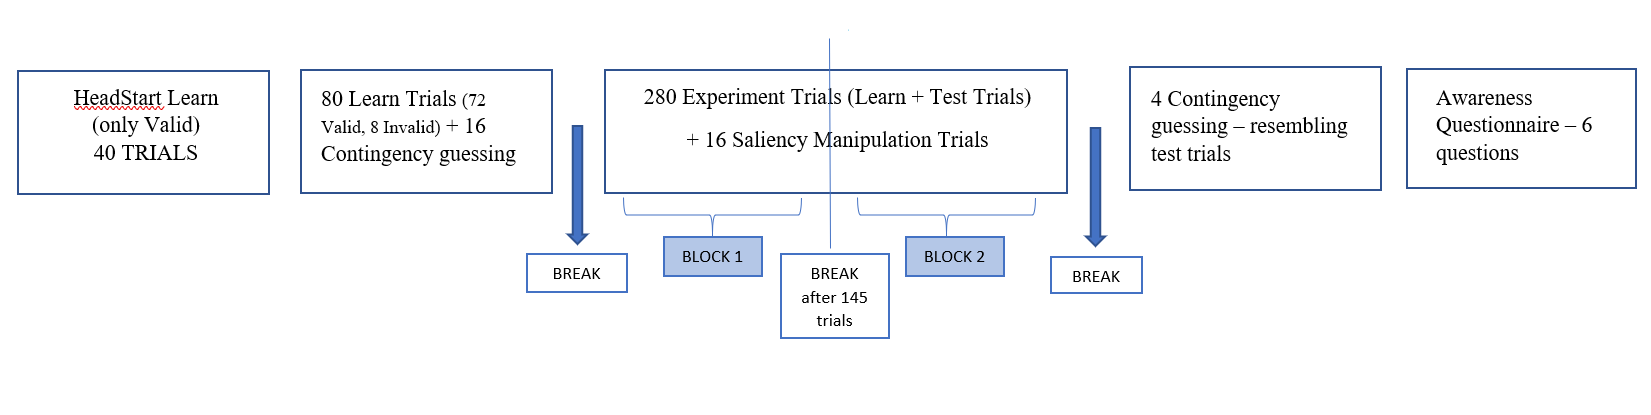
\includegraphics[width=22.93in]{C:/FSU Jena_PhD/Exp7/Experiment-7-Analysis/Figures/Experiment flow}

\emph{The following factors(Distance, Response Type) were computed with
all these trials, without excluding blocks since learn and test trials
were intermixed.}

\hypertarget{data-preparation-and-cleaning}{%
\subsubsection{Data preparation and
cleaning}\label{data-preparation-and-cleaning}}

\begin{itemize}
\tightlist
\item
  Removing unnecessary columns generated by psychopy
\item
  Preparing the RT trial, by eliminating the square brackets and
  splitting it in cases where two keys were registered.
\item
  Creating a column for Accuracy and Error Rate
\item
  adding a Bonus column that computes the points received by each
  participant
\end{itemize}

\begin{Shaded}
\begin{Highlighting}[]
\NormalTok{Exp7data <-}\StringTok{ }\NormalTok{Exp7data }\OperatorTok
\StringTok{  }\KeywordTok{select}\NormalTok{(}\OperatorTok{-}\NormalTok{X,}\OperatorTok{-}\NormalTok{ConsentKey.keys,}\OperatorTok{-}\NormalTok{ConsentKey.rt,}\OperatorTok{-}\NormalTok{Begin.keys,}\OperatorTok{-}\NormalTok{Begin.rt,}\OperatorTok{-}\NormalTok{checkresp.corr,}\OperatorTok{-}\NormalTok{checkresp.keys,}\OperatorTok{-}\NormalTok{checkresp.rt,}\OperatorTok{-}\NormalTok{Attention.thisRepN,}\OperatorTok{-}\NormalTok{Attention.thisTrialN,}\OperatorTok{-}\NormalTok{Attention.thisN,}\OperatorTok{-}\NormalTok{Attention.thisIndex,}\OperatorTok{-}\NormalTok{Attention.ran,}\OperatorTok{-}\NormalTok{AttnQuestion,}\OperatorTok{-}\NormalTok{AttnAnswer,}\OperatorTok{-}\NormalTok{NextStep.keys,}\OperatorTok{-}\NormalTok{NextStep.rt,}\OperatorTok{-}\NormalTok{InstRep.ran,}\OperatorTok{-}\NormalTok{InstRep.thisN,}\OperatorTok{-}\NormalTok{InstRep.thisTrialN,}\OperatorTok{-}\NormalTok{InstRep.thisRepN,}\OperatorTok{-}\NormalTok{InstRep.thisIndex,}\OperatorTok{-}\NormalTok{PracProceed.keys,}\OperatorTok{-}\NormalTok{PracProceed.rt,}\OperatorTok{-}\NormalTok{Prac_loop.thisRepN,}\OperatorTok{-}\NormalTok{Prac_loop.thisTrialN,}\OperatorTok{-}\NormalTok{Prac_loop.thisN,}\OperatorTok{-}\NormalTok{Prac_loop.thisIndex,}\OperatorTok{-}\NormalTok{Prac_loop.ran,}\OperatorTok{-}\NormalTok{Exp_proceed.keys,}\OperatorTok{-}\NormalTok{Exp_proceed.rt,}\OperatorTok{-}\NormalTok{PracRepeat.ran,}\OperatorTok{-}\NormalTok{PracRepeat.thisRepN,}\OperatorTok{-}\NormalTok{PracRepeat.thisN,}\OperatorTok{-}\NormalTok{PracRepeat.thisIndex,}\OperatorTok{-}\NormalTok{PracRepeat.thisTrialN,}\OperatorTok{-}\NormalTok{brkContinue.keys,}\OperatorTok{-}\NormalTok{PauseResp.keys,}\OperatorTok{-}\NormalTok{PauseResp.rt,}\OperatorTok{-}\NormalTok{CALearntrials.thisRepN,}\OperatorTok{-}\NormalTok{CALearntrials.ran,}\OperatorTok{-}\NormalTok{CALearntrials.thisTrialN,}\OperatorTok{-}\NormalTok{CALearntrials.thisIndex, }\OperatorTok{-}\NormalTok{CA_Proceed.keys,}\OperatorTok{-}\NormalTok{CA_Proceed.rt,}\OperatorTok{-}\NormalTok{headstartLearn.thisRepN,}\OperatorTok{-}\NormalTok{headstartLearn.thisTrialN,}\OperatorTok{-}\NormalTok{headstartLearn.thisIndex,}\OperatorTok{-}\NormalTok{headstartLearn.thisN,}\OperatorTok{-}\NormalTok{headstartLearn.ran,}\OperatorTok{-}\NormalTok{ExpTrials.ran,}\OperatorTok{-}\NormalTok{ExpTrials.thisIndex,}\OperatorTok{-}\NormalTok{CA_trials.thisRepN,}\OperatorTok{-}\NormalTok{CA_trials.thisN,}\OperatorTok{-}\NormalTok{CA_trials.thisIndex,}\OperatorTok{-}\NormalTok{CA_trials.thisTrialN,}\OperatorTok{-}\NormalTok{CA_trials.ran,}\OperatorTok{-}\NormalTok{AwareQ_loop.thisRepN,}\OperatorTok{-}\NormalTok{AwareQ_loop.ran,}\OperatorTok{-}\NormalTok{AwareQ_loop.thisIndex,}\OperatorTok{-}\NormalTok{AwareQ_loop.thisTrialN,}\OperatorTok{-}\NormalTok{todebrief.keys,}\OperatorTok{-}\NormalTok{Finalend.keys)}



\CommentTok{#adjusting RT}
\NormalTok{Exp7data}\OperatorTok{$}\NormalTok{mainRT <-}\StringTok{ }\NormalTok{Exp7data}\OperatorTok{$}\NormalTok{TargetResp.rt}
\NormalTok{Exp7data}\OperatorTok{$}\NormalTok{Block1RT <-}\StringTok{ }\NormalTok{Exp7data}\OperatorTok{$}\NormalTok{CAResponse.rt}

\CommentTok{#splitting the RTs from main block}
\NormalTok{Exp7data <-}\StringTok{ }\KeywordTok{separate}\NormalTok{(Exp7data, }\DataTypeTok{col =}\NormalTok{ mainRT, }\DataTypeTok{into =} \KeywordTok{c}\NormalTok{(}\StringTok{"RTm_Trials"}\NormalTok{, }\StringTok{"RTm_secondary"}\NormalTok{), }\DataTypeTok{sep =} \StringTok{','}\NormalTok{)}
\NormalTok{Exp7data}\OperatorTok{$}\NormalTok{RTm_Trials <-}\StringTok{ }\NormalTok{Exp7data}\OperatorTok{$}\NormalTok{RTm_Trials}\OperatorTok
\StringTok{  }\KeywordTok{str_replace_all}\NormalTok{(}\StringTok{"}\CharTok{\textbackslash{}\textbackslash{}}\StringTok{[|}\CharTok{\textbackslash{}\textbackslash{}}\StringTok{]"}\NormalTok{,}\StringTok{""}\NormalTok{)}\OperatorTok
\StringTok{  }\KeywordTok{as.double}\NormalTok{(Exp7data}\OperatorTok{$}\NormalTok{RTm_Trials)}
\NormalTok{Exp7data}\OperatorTok{$}\NormalTok{RTm_Trials <-}\StringTok{ }\DecValTok{1000}\OperatorTok{*}\NormalTok{(Exp7data}\OperatorTok{$}\NormalTok{RTm_Trials)}

\CommentTok{#splitting RTs from the Ca learn block (1st block)}
\NormalTok{Exp7data <-}\StringTok{ }\KeywordTok{separate}\NormalTok{(Exp7data, }\DataTypeTok{col =}\NormalTok{ Block1RT, }\DataTypeTok{into =} \KeywordTok{c}\NormalTok{(}\StringTok{"RTb_Trials"}\NormalTok{, }\StringTok{"RTb_secondary"}\NormalTok{), }\DataTypeTok{sep =} \StringTok{','}\NormalTok{)}
\NormalTok{Exp7data}\OperatorTok{$}\NormalTok{RTb_Trials <-}\StringTok{ }\NormalTok{Exp7data}\OperatorTok{$}\NormalTok{RTb_Trials}\OperatorTok
\StringTok{  }\KeywordTok{str_replace_all}\NormalTok{(}\StringTok{"}\CharTok{\textbackslash{}\textbackslash{}}\StringTok{[|}\CharTok{\textbackslash{}\textbackslash{}}\StringTok{]"}\NormalTok{,}\StringTok{""}\NormalTok{)}\OperatorTok
\StringTok{  }\KeywordTok{as.double}\NormalTok{(Exp7data}\OperatorTok{$}\NormalTok{RTb_Trials)}
\NormalTok{Exp7data}\OperatorTok{$}\NormalTok{RTb_Trials <-}\StringTok{ }\DecValTok{1000}\OperatorTok{*}\NormalTok{(Exp7data}\OperatorTok{$}\NormalTok{RTb_Trials)}

\CommentTok{#removing RTs from guessing trials }
\NormalTok{Exp7data}\OperatorTok{$}\NormalTok{RTb_Trials <-}\StringTok{ }\KeywordTok{ifelse}\NormalTok{(Exp7data}\OperatorTok{$}\NormalTok{Block }\OperatorTok{==}\StringTok{ "CG Learn"}\NormalTok{, }\OtherTok{NA}\NormalTok{, Exp7data}\OperatorTok{$}\NormalTok{RTb_Trials)}

\CommentTok{#creating a dummy variable to pick wherever the RTs are from main block and which are from first block}
\NormalTok{Exp7data}\OperatorTok{$}\NormalTok{RTdummy <-}\StringTok{ }\KeywordTok{ifelse}\NormalTok{(}\KeywordTok{is.na}\NormalTok{(Exp7data}\OperatorTok{$}\NormalTok{TargetResp.rt) }\OperatorTok{==}\StringTok{ }\OtherTok{FALSE}\NormalTok{,}\DecValTok{1}\NormalTok{,}\OtherTok{NA}\NormalTok{)}
\NormalTok{Exp7data}\OperatorTok{$}\NormalTok{RTdummy <-}\StringTok{ }\KeywordTok{ifelse}\NormalTok{(}\KeywordTok{is.na}\NormalTok{(Exp7data}\OperatorTok{$}\NormalTok{CAResponse.rt)}\OperatorTok{==}\OtherTok{FALSE}\NormalTok{,}\DecValTok{2}\NormalTok{,Exp7data}\OperatorTok{$}\NormalTok{RTdummy)}

\CommentTok{#combining all important RTs }
\NormalTok{Exp7data <-}\StringTok{ }\NormalTok{Exp7data }\OperatorTok
\StringTok{  }\KeywordTok{mutate}\NormalTok{(}\DataTypeTok{RT_Trials =} \KeywordTok{ifelse}\NormalTok{((RTdummy }\OperatorTok{==}\StringTok{ }\DecValTok{1}\NormalTok{), RTm_Trials,}\KeywordTok{ifelse}\NormalTok{((RTdummy }\OperatorTok{==}\StringTok{ }\DecValTok{2}\NormalTok{),RTb_Trials,}\OtherTok{NA}\NormalTok{)))}


\CommentTok{###creating a separate df with the contingency awareness}
\NormalTok{Exp7_CA <-}\StringTok{ }\NormalTok{Exp7data}\OperatorTok
\StringTok{  }\KeywordTok{filter}\NormalTok{(Target }\OperatorTok{==}\StringTok{ "?"} \OperatorTok{|}\StringTok{ }\KeywordTok{str_detect}\NormalTok{(AwareQ, }\StringTok{"Press"}\NormalTok{))}





\NormalTok{Exp7data <-}\StringTok{ }\NormalTok{Exp7data}\OperatorTok\KeywordTok{drop_na}\NormalTok{(RT_Trials)}

\CommentTok{#combining accuracy from first block and main block}
\NormalTok{Exp7data}\OperatorTok{$}\NormalTok{mainAcc <-}\StringTok{ }\NormalTok{Exp7data}\OperatorTok{$}\NormalTok{TargetResp.corr}
\NormalTok{Exp7data}\OperatorTok{$}\NormalTok{Block1Acc <-}\StringTok{ }\NormalTok{Exp7data}\OperatorTok{$}\NormalTok{CAResponse.corr}
\NormalTok{Exp7data}\OperatorTok{$}\NormalTok{BlockAcc <-}\StringTok{ }\KeywordTok{ifelse}\NormalTok{(Exp7data}\OperatorTok{$}\NormalTok{Block }\OperatorTok{==}\StringTok{ "CG Learn"}\NormalTok{, }\OtherTok{NA}\NormalTok{, Exp7data}\OperatorTok{$}\NormalTok{Block1Acc)}

\NormalTok{Exp7data}\OperatorTok{$}\NormalTok{ACCdummy <-}\StringTok{ }\KeywordTok{ifelse}\NormalTok{(}\KeywordTok{is.na}\NormalTok{(Exp7data}\OperatorTok{$}\NormalTok{TargetResp.corr)}\OperatorTok{==}\OtherTok{FALSE}\NormalTok{,}\DecValTok{1}\NormalTok{,}\OtherTok{NA}\NormalTok{)}
\NormalTok{Exp7data}\OperatorTok{$}\NormalTok{ACCdummy <-}\StringTok{ }\KeywordTok{ifelse}\NormalTok{(}\KeywordTok{is.na}\NormalTok{(Exp7data}\OperatorTok{$}\NormalTok{CAResponse.corr)}\OperatorTok{==}\OtherTok{FALSE}\NormalTok{,}\DecValTok{2}\NormalTok{,Exp7data}\OperatorTok{$}\NormalTok{ACCdummy)}

\NormalTok{Exp7data <-}\StringTok{ }\NormalTok{Exp7data }\OperatorTok
\StringTok{  }\KeywordTok{mutate}\NormalTok{(}\DataTypeTok{ACC_trials =} \KeywordTok{ifelse}\NormalTok{((ACCdummy }\OperatorTok{==}\StringTok{ }\DecValTok{1}\NormalTok{),mainAcc,}\KeywordTok{ifelse}\NormalTok{((ACCdummy }\OperatorTok{==}\StringTok{ }\DecValTok{2}\NormalTok{),Block1Acc,}\OtherTok{NA}\NormalTok{)))}


\NormalTok{Exp7data}\OperatorTok{$}\NormalTok{ErrorRate <-}\StringTok{ }\DecValTok{1} \OperatorTok{-}\StringTok{ }\NormalTok{Exp7data}\OperatorTok{$}\NormalTok{ACC_trials}

\CommentTok{#Error rate}
\KeywordTok{pander}\NormalTok{(}\KeywordTok{table}\NormalTok{(Exp7data}\OperatorTok{$}\NormalTok{ACC_trials), }\DataTypeTok{style =} \StringTok{"rmarkdown"}\NormalTok{, }\DataTypeTok{caption =} \StringTok{"Total number of Accuracy trials"}\NormalTok{)}
\end{Highlighting}
\end{Shaded}

\begin{longtable}[]{@{}cc@{}}
\caption{Total number of Accuracy trials}\tabularnewline
\toprule
0 & 1\tabularnewline
\midrule
\endfirsthead
\toprule
0 & 1\tabularnewline
\midrule
\endhead
1982 & 27554\tabularnewline
\bottomrule
\end{longtable}

\begin{Shaded}
\begin{Highlighting}[]
\KeywordTok{pander}\NormalTok{(}\KeywordTok{round}\NormalTok{(}\KeywordTok{table}\NormalTok{(Exp7data}\OperatorTok{$}\NormalTok{ACC_trials)}\OperatorTok{/}\KeywordTok{nrow}\NormalTok{(Exp7data)}\OperatorTok{*}\DecValTok{100}\NormalTok{, }\DataTypeTok{digits =} \DecValTok{3}\NormalTok{), }\DataTypeTok{style =} \StringTok{"rmarkdown"}\NormalTok{,}\DataTypeTok{caption =} \StringTok{"Percentage of accuracy and errors"}\NormalTok{)}
\end{Highlighting}
\end{Shaded}

\begin{longtable}[]{@{}cc@{}}
\caption{Percentage of accuracy and errors}\tabularnewline
\toprule
0 & 1\tabularnewline
\midrule
\endfirsthead
\toprule
0 & 1\tabularnewline
\midrule
\endhead
6.71 & 93.29\tabularnewline
\bottomrule
\end{longtable}

Upon implementing the exclusion criteria

\begin{itemize}
\tightlist
\item
  Outliers (1.5x above third quartile) --\textgreater{} used for the
  analysis
\item
  Farouts (3x)above third quartile)
\item
  very Fast RTs, less than 200ms
\end{itemize}

\begin{Shaded}
\begin{Highlighting}[]
\CommentTok{#Exclude errors from RT}
\NormalTok{Exp7data <-}\StringTok{ }\NormalTok{Exp7data }\OperatorTok
\StringTok{  }\KeywordTok{filter}\NormalTok{(participant }\OperatorTok{!=}\StringTok{ }\DecValTok{10}\NormalTok{)}
\NormalTok{Exp7data}\OperatorTok{$}\NormalTok{RT_Trials[Exp7data}\OperatorTok{$}\NormalTok{ACC_trials}\OperatorTok{==}\DecValTok{0}\NormalTok{] <-}\StringTok{ }\OtherTok{NA}
\KeywordTok{pander}\NormalTok{(}\KeywordTok{summary}\NormalTok{(Exp7data}\OperatorTok{$}\NormalTok{RT_Trials), }\DataTypeTok{style =} \StringTok{"rmarkdown"}\NormalTok{, }\DataTypeTok{caption =} \StringTok{"Mean of RTs before exclusions"}\NormalTok{)}
\end{Highlighting}
\end{Shaded}

\begin{longtable}[]{@{}ccccccc@{}}
\caption{Mean of RTs before exclusions}\tabularnewline
\toprule
Min. & 1st Qu. & Median & Mean & 3rd Qu. & Max. & NA's\tabularnewline
\midrule
\endfirsthead
\toprule
Min. & 1st Qu. & Median & Mean & 3rd Qu. & Max. & NA's\tabularnewline
\midrule
\endhead
1.505 & 467.9 & 561 & 602.1 & 673.5 & 8581 & 1867\tabularnewline
\bottomrule
\end{longtable}

\begin{Shaded}
\begin{Highlighting}[]
\CommentTok{#exclude outliers}
\CommentTok{#creating function to remove the outliers and farouts}
\NormalTok{computeTukeys <-}\StringTok{ }\ControlFlowTok{function}\NormalTok{(x)\{}
\NormalTok{  P25 <-}\StringTok{ }\KeywordTok{quantile}\NormalTok{(x}\OperatorTok{$}\NormalTok{RT_Trials, }\FloatTok{.25}\NormalTok{, }\DataTypeTok{na.rm =} \OtherTok{TRUE}\NormalTok{, }\DataTypeTok{type =} \DecValTok{6}\NormalTok{) }\CommentTok{#type = 6 -> used in SPSS}
\NormalTok{  P75 <-}\StringTok{ }\KeywordTok{quantile}\NormalTok{(x}\OperatorTok{$}\NormalTok{RT_Trials, }\FloatTok{.75}\NormalTok{, }\DataTypeTok{na.rm =} \OtherTok{TRUE}\NormalTok{, }\DataTypeTok{type =} \DecValTok{6}\NormalTok{)}
\NormalTok{  x}\OperatorTok{$}\NormalTok{Outlier <-}\StringTok{ }\NormalTok{P75 }\OperatorTok{+}\StringTok{ }\FloatTok{1.5}\OperatorTok{*}\NormalTok{(P75 }\OperatorTok{-}\StringTok{ }\NormalTok{P25)}
\NormalTok{  x}\OperatorTok{$}\NormalTok{Farouts <-}\StringTok{ }\NormalTok{P75 }\OperatorTok{+}\StringTok{ }\FloatTok{3.0}\OperatorTok{*}\NormalTok{(P75 }\OperatorTok{-}\StringTok{ }\NormalTok{P25)}
  \KeywordTok{return}\NormalTok{(x)}
\NormalTok{\}}


\CommentTok{#identifying the outliers and farouts at individual level}
\NormalTok{Exp7data <-}\StringTok{ }\KeywordTok{ddply}\NormalTok{(Exp7data, .(participant), computeTukeys)}

\CommentTok{#creating new column with RT trials after removing outliers/farouts}
\NormalTok{Exp7data}\OperatorTok{$}\NormalTok{RT_io <-}\StringTok{ }\NormalTok{Exp7data}\OperatorTok{$}\NormalTok{RT_Trials}

\NormalTok{Exp7data}\OperatorTok{$}\NormalTok{RT_io[Exp7data}\OperatorTok{$}\NormalTok{RT_io }\OperatorTok{>}\StringTok{ }\NormalTok{Exp7data}\OperatorTok{$}\NormalTok{Outlier}\OperatorTok{|}\NormalTok{Exp7data}\OperatorTok{$}\NormalTok{RT_io }\OperatorTok{<}\StringTok{ }\DecValTok{200}\NormalTok{] <-}\StringTok{ }\OtherTok{NA}
\KeywordTok{pander}\NormalTok{(}\KeywordTok{summary}\NormalTok{(Exp7data}\OperatorTok{$}\NormalTok{RT_io), }\DataTypeTok{style =} \StringTok{"rmarkdown"}\NormalTok{, }\DataTypeTok{caption =} \StringTok{"Mean RTs after removing outliers"}\NormalTok{)}
\end{Highlighting}
\end{Shaded}

\begin{longtable}[]{@{}ccccccc@{}}
\caption{Mean RTs after removing outliers}\tabularnewline
\toprule
Min. & 1st Qu. & Median & Mean & 3rd Qu. & Max. & NA's\tabularnewline
\midrule
\endfirsthead
\toprule
Min. & 1st Qu. & Median & Mean & 3rd Qu. & Max. & NA's\tabularnewline
\midrule
\endhead
200.3 & 465.7 & 553.4 & 571.3 & 653.5 & 1733 & 3350\tabularnewline
\bottomrule
\end{longtable}

\hypertarget{previous-occurence-analysis-distance-response-type}{%
\subsection{Previous Occurence Analysis : Distance \& Response
Type}\label{previous-occurence-analysis-distance-response-type}}

\hypertarget{distance}{%
\subsubsection{1. Distance}\label{distance}}

This variable tells how far ago the last occurence of distractor appear

The conditions used for these in comparsion to current trial \(n\)
within participant were as follows:

\begin{enumerate}
\def\labelenumi{\arabic{enumi}.}
\tightlist
\item
  whether Trial \(n-1\) or \(n-x\) was a \emph{learn} or a \emph{test}
  trial.
\item
  if either the Salient Distractor or Non salient Distractor appeared in
  Trial \(n-1\) or \(n-x\)
\item
  if Trial \(n-1\) / \(n-x\) was an accurate trial
\end{enumerate}

and \(x\) was saved as the Distance variable if it satisified
\textbf{all} the above conditions where \(x\) refers to the xth number
of the trial behind \(n\)

\begin{Shaded}
\begin{Highlighting}[]
\CommentTok{#add previous_respoonse and distance to the model####}
\NormalTok{Exp7data <-}\StringTok{ }\NormalTok{Exp7data}\OperatorTok\KeywordTok{select}\NormalTok{(Condition, SalD,NSalD,Saliency,Validity, }\KeywordTok{everything}\NormalTok{())}

\CommentTok{###first is to find out the trials where the previous occurence wa the immediate previous one}
\NormalTok{Exp7data}\OperatorTok{$}\NormalTok{Distance <-}\StringTok{ }\OtherTok{NA}
\NormalTok{Exp7data <-}\StringTok{ }\NormalTok{Exp7data}\OperatorTok\KeywordTok{select}\NormalTok{(Distance,ACC_trials,}\KeywordTok{everything}\NormalTok{())}
\NormalTok{Exp7data <-}\StringTok{ }\NormalTok{Exp7data}\OperatorTok
\StringTok{  }\KeywordTok{mutate}\NormalTok{(}\DataTypeTok{Distance =} \KeywordTok{ifelse}\NormalTok{((}\KeywordTok{lag}\NormalTok{(Condition,}\DecValTok{1}\NormalTok{)}\OperatorTok{==}\StringTok{"test"} \OperatorTok{|}\StringTok{ }\KeywordTok{lag}\NormalTok{(Condition,}\DecValTok{1}\NormalTok{) }\OperatorTok{==}\StringTok{ "learn"}\NormalTok{)}\OperatorTok{&}\StringTok{ }
\StringTok{                             }\NormalTok{(}\KeywordTok{lag}\NormalTok{(SalD,}\DecValTok{1}\NormalTok{)}\OperatorTok{==}\StringTok{ }\NormalTok{SalD}\OperatorTok{|}\KeywordTok{lag}\NormalTok{(NSalD,}\DecValTok{1}\NormalTok{)}\OperatorTok{==}\NormalTok{NSalD) }\OperatorTok{&}
\StringTok{                             }\KeywordTok{lag}\NormalTok{(participant,}\DecValTok{1}\NormalTok{)}\OperatorTok{==}\NormalTok{participant }\OperatorTok{&}
\StringTok{                             }\KeywordTok{lag}\NormalTok{(ACC_trials,}\DecValTok{1}\NormalTok{)}\OperatorTok{==}\StringTok{ }\DecValTok{1}\NormalTok{, }\DecValTok{1}\NormalTok{, Distance))}


\CommentTok{#The number of immediate previous occurences}

\KeywordTok{pander}\NormalTok{(}\KeywordTok{table}\NormalTok{(Exp7data}\OperatorTok{$}\NormalTok{Distance), }\DataTypeTok{style =} \StringTok{"rmarkdown"}\NormalTok{, }\DataTypeTok{caption =} \StringTok{"Number of immediately preceding previous occurences"}\NormalTok{)}
\end{Highlighting}
\end{Shaded}

\begin{longtable}[]{@{}c@{}}
\caption{Number of immediately preceding previous
occurences}\tabularnewline
\toprule
1\tabularnewline
\midrule
\endfirsthead
\toprule
1\tabularnewline
\midrule
\endhead
12668\tabularnewline
\bottomrule
\end{longtable}

\begin{Shaded}
\begin{Highlighting}[]
\CommentTok{## Now to look at other distances of the last occurrence beyond the immediately preceding one}
\NormalTok{lagvalue <-}\StringTok{ }\DecValTok{2}\OperatorTok{:}\DecValTok{20}

\ControlFlowTok{for}\NormalTok{(j }\ControlFlowTok{in}\NormalTok{ lagvalue)\{}
\NormalTok{  Exp7data <-}\StringTok{ }\NormalTok{Exp7data }\OperatorTok\StringTok{ }
\StringTok{    }\KeywordTok{mutate}\NormalTok{(}\DataTypeTok{Distance =} \KeywordTok{ifelse}\NormalTok{((}\KeywordTok{lag}\NormalTok{(Condition,j)}\OperatorTok{==}\StringTok{"learn"}\OperatorTok{|}\KeywordTok{lag}\NormalTok{(Condition,j)}\OperatorTok{==}\StringTok{"test"}\NormalTok{) }\OperatorTok{&}\StringTok{  }
\StringTok{                             }\NormalTok{(}\KeywordTok{lag}\NormalTok{(SalD,j)}\OperatorTok{==}\NormalTok{SalD}\OperatorTok{|}\KeywordTok{lag}\NormalTok{(NSalD,j)}\OperatorTok{==}\NormalTok{NSalD) }\OperatorTok{&}\StringTok{ }\KeywordTok{lag}\NormalTok{(participant,j)}\OperatorTok{==}\NormalTok{participant }\OperatorTok{&}
\StringTok{                              }\KeywordTok{lag}\NormalTok{(ACC_trials,j)}\OperatorTok{==}\StringTok{ }\DecValTok{1} \OperatorTok{&}\StringTok{ }\KeywordTok{is.na}\NormalTok{(Distance)}\OperatorTok{==}\OtherTok{TRUE}\NormalTok{, j, Distance))}
\NormalTok{\}}

\KeywordTok{pander}\NormalTok{(}\KeywordTok{table}\NormalTok{(Exp7data}\OperatorTok{$}\NormalTok{Distance), }\DataTypeTok{style =} \StringTok{"rmarkdown"}\NormalTok{, }\DataTypeTok{caption =} \StringTok{"Number of previous occurences at each distance"}\NormalTok{)}
\end{Highlighting}
\end{Shaded}

\begin{longtable}[]{@{}ccccccccccc@{}}
\caption{Number of previous occurences at each distance (continued
below)}\tabularnewline
\toprule
1 & 2 & 3 & 4 & 5 & 6 & 7 & 8 & 9 & 10 & 11\tabularnewline
\midrule
\endfirsthead
\toprule
1 & 2 & 3 & 4 & 5 & 6 & 7 & 8 & 9 & 10 & 11\tabularnewline
\midrule
\endhead
12668 & 7618 & 4196 & 2091 & 1096 & 592 & 318 & 179 & 106 & 47 &
16\tabularnewline
\bottomrule
\end{longtable}

\begin{longtable}[]{@{}cccccc@{}}
\toprule
12 & 13 & 14 & 15 & 16 & 17\tabularnewline
\midrule
\endhead
17 & 13 & 5 & 4 & 1 & 1\tabularnewline
\bottomrule
\end{longtable}

\hypertarget{previous-response}{%
\subsubsection{2. Previous Response}\label{previous-response}}

Coding what the previous Response was, whether it was the same or
different. This variable is defined as Response Type, which has two
factors: Response Change(RC) and Response Repetition (RR)

This variable is computed based on the following conditions (only with
respect to Trial \(n\) and Trial \(n-1\)):

\begin{enumerate}
\def\labelenumi{\arabic{enumi}.}
\tightlist
\item
  whether the previous trial was \emph{learn} or a \emph{test} trial
\item
  whether the same Salient or Nonsalient Distractor appeared in both
  Trial \(n\) and Trial \(n-1\)
\item
  Whether the Correct Answer for Trial\(n-1\) is same as Trial \(n\)
  (then RR) or different from Trial \(n\) (then RC)
\end{enumerate}

\emph{To be noted: This does not equate to validity} because the SRB
trials can have the combination of invalid prime and invalid probe
--\textgreater{} Response Repetition which is confounded by Validity. So
every valid probe can have both the Response Type factors based on
whether the prime is valid or invalid

\begin{Shaded}
\begin{Highlighting}[]
\NormalTok{Exp7data}\OperatorTok{$}\NormalTok{ResponseType <-}\StringTok{ }\OtherTok{NA}

\NormalTok{Rmlag <-}\StringTok{ }\DecValTok{1}\OperatorTok{:}\DecValTok{30}
\ControlFlowTok{for}\NormalTok{(k }\ControlFlowTok{in}\NormalTok{ Rmlag)\{}
\NormalTok{  Exp7data <-}\StringTok{ }\NormalTok{Exp7data }\OperatorTok\StringTok{ }
\StringTok{    }\KeywordTok{mutate}\NormalTok{(}\DataTypeTok{ResponseType =} \KeywordTok{ifelse}\NormalTok{((}\KeywordTok{lag}\NormalTok{(Condition,k)}\OperatorTok{==}\StringTok{"learn"} \OperatorTok{|}\StringTok{ }\KeywordTok{lag}\NormalTok{(Condition,k)}\OperatorTok{==}\StringTok{"test"}\NormalTok{) }\OperatorTok{&}\StringTok{  }
\StringTok{                                   }\NormalTok{(}\KeywordTok{lag}\NormalTok{(SalD,k)}\OperatorTok{==}\NormalTok{SalD}\OperatorTok{|}\KeywordTok{lag}\NormalTok{(NSalD,k)}\OperatorTok{==}\NormalTok{NSalD) }\OperatorTok{&}\StringTok{ }\KeywordTok{lag}\NormalTok{(participant,k)}\OperatorTok{==}\NormalTok{participant }\OperatorTok{&}\StringTok{ }
\StringTok{                                   }\KeywordTok{lag}\NormalTok{(CorrectAnswer,k)}\OperatorTok{==}\StringTok{ }\NormalTok{CorrectAnswer }\OperatorTok{&}\StringTok{ }\KeywordTok{is.na}\NormalTok{(ResponseType)}\OperatorTok{==}\OtherTok{TRUE}\NormalTok{, }\StringTok{"RR"}\NormalTok{, }
                                 \KeywordTok{ifelse}\NormalTok{((}\KeywordTok{lag}\NormalTok{(Condition,k)}\OperatorTok{==}\StringTok{"learn"}\OperatorTok{|}\KeywordTok{lag}\NormalTok{(Condition,k)}\OperatorTok{==}\StringTok{"test"}\NormalTok{) }\OperatorTok{&}\StringTok{ }\NormalTok{(}\KeywordTok{lag}\NormalTok{(SalD,k)}\OperatorTok{==}\NormalTok{SalD}\OperatorTok{|}\KeywordTok{lag}\NormalTok{(NSalD,k)}\OperatorTok{==}\NormalTok{NSalD)}\OperatorTok{&}\StringTok{ }\KeywordTok{lag}\NormalTok{(participant,k)}\OperatorTok{==}\NormalTok{participant }\OperatorTok{&}\StringTok{ }\KeywordTok{lag}\NormalTok{(CorrectAnswer,k)}\OperatorTok{!=}\StringTok{ }\NormalTok{CorrectAnswer }\OperatorTok{&}\StringTok{ }\KeywordTok{is.na}\NormalTok{(ResponseType)}\OperatorTok{==}\OtherTok{TRUE}\NormalTok{, }\StringTok{"RC"}\NormalTok{, ResponseType)))}
\NormalTok{\}}

\KeywordTok{pander}\NormalTok{(}\KeywordTok{table}\NormalTok{(Exp7data}\OperatorTok{$}\NormalTok{ResponseType),}\DataTypeTok{style =} \StringTok{"rmarkdown"}\NormalTok{, }\DataTypeTok{caption =} \StringTok{"Number of Response Repetitions and Change"}\NormalTok{)}
\end{Highlighting}
\end{Shaded}

\begin{longtable}[]{@{}cc@{}}
\caption{Number of Response Repetitions and Change}\tabularnewline
\toprule
RC & RR\tabularnewline
\midrule
\endfirsthead
\toprule
RC & RR\tabularnewline
\midrule
\endhead
7777 & 21203\tabularnewline
\bottomrule
\end{longtable}

\begin{Shaded}
\begin{Highlighting}[]
\NormalTok{Exp7data <-}\StringTok{ }\NormalTok{Exp7data}\OperatorTok\KeywordTok{select}\NormalTok{(ResponseType,RT_io,CorrectAnswer, }\KeywordTok{everything}\NormalTok{())}
\end{Highlighting}
\end{Shaded}

\hypertarget{multi-level-modelling}{%
\section{MULTI LEVEL MODELLING}\label{multi-level-modelling}}

\begin{enumerate}
\def\labelenumi{\arabic{enumi}.}
\tightlist
\item
  Creating a dataframe copying the entire dataset with all 70
  participants and all the conditions.
\item
  Changing the predictor levels to numeric type
\end{enumerate}

\begin{itemize}
\tightlist
\item
  Validity --\textgreater{} Val = 1,2 (valid, invalid)
\item
  ResponseType --\textgreater{} previous\_rm = 1,2 (RR,RC)
\item
  Distance is already numeric
\end{itemize}

\begin{enumerate}
\def\labelenumi{\arabic{enumi}.}
\setcounter{enumi}{2}
\tightlist
\item
  creating a standardised score for the predictors: ZVal, Zprevious\_rm,
  zDistance
\end{enumerate}

\begin{Shaded}
\begin{Highlighting}[]
\CommentTok{#Compute first model: level1 predictor: probe compatiblity; level2 predictor: subject;}
\CommentTok{#random slopes, predict RT with contingency factor (high vs low) = aka "probe_comp" var ####}


\NormalTok{raw.data<-Exp7data}

\CommentTok{#compute new numeric var for validity effect}
\NormalTok{raw.data}\OperatorTok{$}\NormalTok{val <-}\KeywordTok{ifelse}\NormalTok{(raw.data}\OperatorTok{$}\NormalTok{Validity}\OperatorTok{==}\StringTok{"valid"}\NormalTok{,}\DecValTok{1}\NormalTok{,}\DecValTok{2}\NormalTok{)}
\KeywordTok{pander}\NormalTok{(}\KeywordTok{table}\NormalTok{(raw.data}\OperatorTok{$}\NormalTok{Validity,raw.data}\OperatorTok{$}\NormalTok{val), }\DataTypeTok{style =} \StringTok{"rmarkdown"}\NormalTok{, }\DataTypeTok{caption =} \StringTok{"Numeric values of validity"}\NormalTok{)}
\end{Highlighting}
\end{Shaded}

\begin{longtable}[]{@{}ccc@{}}
\caption{Numeric values of validity}\tabularnewline
\toprule
~ & 1 & 2\tabularnewline
\midrule
\endfirsthead
\toprule
~ & 1 & 2\tabularnewline
\midrule
\endhead
\textbf{invalid} & 0 & 4760\tabularnewline
\textbf{valid} & 24360 & 0\tabularnewline
\bottomrule
\end{longtable}

\begin{Shaded}
\begin{Highlighting}[]
\CommentTok{#create numerical var for response type}

\NormalTok{raw.data}\OperatorTok{$}\NormalTok{previous_rm<-}\KeywordTok{ifelse}\NormalTok{(raw.data}\OperatorTok{$}\NormalTok{ResponseType}\OperatorTok{==}\StringTok{"RR"}\NormalTok{, }\DecValTok{1}\NormalTok{, }\DecValTok{2}\NormalTok{)}
\KeywordTok{pander}\NormalTok{(}\KeywordTok{table}\NormalTok{(raw.data}\OperatorTok{$}\NormalTok{ResponseType, raw.data}\OperatorTok{$}\NormalTok{previous_rm), }\DataTypeTok{style =} \StringTok{"rmarkdown"}\NormalTok{, }\DataTypeTok{caption =} \StringTok{"Numeric values of Response Type"}\NormalTok{)}
\end{Highlighting}
\end{Shaded}

\begin{longtable}[]{@{}ccc@{}}
\caption{Numeric values of Response Type}\tabularnewline
\toprule
~ & 1 & 2\tabularnewline
\midrule
\endfirsthead
\toprule
~ & 1 & 2\tabularnewline
\midrule
\endhead
\textbf{RC} & 0 & 7777\tabularnewline
\textbf{RR} & 21203 & 0\tabularnewline
\bottomrule
\end{longtable}

\begin{Shaded}
\begin{Highlighting}[]
\CommentTok{#center predictors}

\NormalTok{raw.data}\OperatorTok{$}\NormalTok{Zval=}\KeywordTok{scale}\NormalTok{(raw.data}\OperatorTok{$}\NormalTok{val, }\DataTypeTok{scale=}\OtherTok{FALSE}\NormalTok{)}
\NormalTok{raw.data}\OperatorTok{$}\NormalTok{Zprevious_rm=}\KeywordTok{scale}\NormalTok{(raw.data}\OperatorTok{$}\NormalTok{previous_rm, }\DataTypeTok{scale=}\NormalTok{F)}
\NormalTok{raw.data}\OperatorTok{$}\NormalTok{ZDistance=}\KeywordTok{scale}\NormalTok{(raw.data}\OperatorTok{$}\NormalTok{Distance, }\DataTypeTok{scale=}\NormalTok{F)}

\KeywordTok{summary}\NormalTok{(raw.data}\OperatorTok{$}\NormalTok{Distance)}
\end{Highlighting}
\end{Shaded}

\begin{verbatim}
##    Min. 1st Qu.  Median    Mean 3rd Qu.    Max.    NA's 
##   1.000   1.000   2.000   2.198   3.000  17.000     152
\end{verbatim}

\hypertarget{model-1-only-with-validity-as-level-1-predictor-with-intercept-varying-over-participant}{%
\subsection{1. Model 1: Only with Validity as Level 1 Predictor with
intercept varying over
participant}\label{model-1-only-with-validity-as-level-1-predictor-with-intercept-varying-over-participant}}

\begin{quote}
Validity has a significant effect
\end{quote}

This contains the valid and invalid trials across the whole experiment
including learn and test.

\begin{Shaded}
\begin{Highlighting}[]
\NormalTok{randomSlopes_m1<-}\KeywordTok{lmer}\NormalTok{(RT_io}\OperatorTok{~}\DecValTok{1}\OperatorTok{+}\NormalTok{val }\OperatorTok{+}\StringTok{ }\NormalTok{(}\DecValTok{1}\OperatorTok{+}\NormalTok{val}\OperatorTok{|}\NormalTok{participant), }
                      \DataTypeTok{data=}\NormalTok{raw.data, }
                      \DataTypeTok{REML=}\NormalTok{F,}
                      \DataTypeTok{na.action =} \StringTok{"na.omit"}\NormalTok{)}



\NormalTok{sjPlot}\OperatorTok{::}\KeywordTok{tab_model}\NormalTok{(randomSlopes_m1, }\DataTypeTok{show.se =} \OtherTok{TRUE}\NormalTok{,}\DataTypeTok{show.stat =} \OtherTok{TRUE}\NormalTok{, }\DataTypeTok{show.ci =} \OtherTok{FALSE}\NormalTok{, }
                  \DataTypeTok{pred.labels =} \KeywordTok{c}\NormalTok{(}\StringTok{"Intercept"}\NormalTok{,}\StringTok{"Validity"}\NormalTok{),}
                  \DataTypeTok{dv.labels =} \StringTok{"Reaction Time"}\NormalTok{)}
\end{Highlighting}
\end{Shaded}

~

Reaction Time

Predictors

Estimates

std. Error

Statistic

p

Intercept

536.74

13.48

39.81

\textless0.001

Validity

29.78

4.56

6.53

\textless0.001

Random Effects

σ2

18864.84

τ00 participant

12139.44

τ11 participant.val

1053.20

ρ01 participant

-0.73

ICC

0.29

N participant

70

Observations

25770

Marginal R2 / Conditional R2

0.004 / 0.293

\begin{Shaded}
\begin{Highlighting}[]
\KeywordTok{summary}\NormalTok{(randomSlopes_m1)}
\end{Highlighting}
\end{Shaded}

\begin{verbatim}
## Linear mixed model fit by maximum likelihood . t-tests use Satterthwaite's
##   method [lmerModLmerTest]
## Formula: RT_io ~ 1 + val + (1 + val | participant)
##    Data: raw.data
## 
##       AIC       BIC    logLik  deviance  df.resid 
##  327278.1  327327.0 -163633.0  327266.1     25764 
## 
## Scaled residuals: 
##     Min      1Q  Median      3Q     Max 
## -3.8007 -0.6526 -0.0994  0.5391  6.4988 
## 
## Random effects:
##  Groups      Name        Variance Std.Dev. Corr 
##  participant (Intercept) 12139    110.18        
##              val          1053     32.45   -0.73
##  Residual                18865    137.35        
## Number of obs: 25770, groups:  participant, 70
## 
## Fixed effects:
##             Estimate Std. Error     df t value Pr(>|t|)    
## (Intercept)   536.74      13.48  69.88  39.812  < 2e-16 ***
## val            29.78       4.56  69.17   6.531 9.23e-09 ***
## ---
## Signif. codes:  0 '***' 0.001 '**' 0.01 '*' 0.05 '.' 0.1 ' ' 1
## 
## Correlation of Fixed Effects:
##     (Intr)
## val -0.711
\end{verbatim}

\hypertarget{model-2-adding-the-factors-of-previous-response-rr-or-rc-to-the-previous-model}{%
\subsection{2. Model 2: Adding the Factors of Previous Response (RR or
RC) to the previous
model}\label{model-2-adding-the-factors-of-previous-response-rr-or-rc-to-the-previous-model}}

Using the standardised scores of the predictors (\emph{centering is not
effective- RR and RC are not equal in number})

This also includes trials that are both learn and test, both invalid and
valid.

\begin{Shaded}
\begin{Highlighting}[]
\NormalTok{randomSlopes_m2<-}\KeywordTok{lmer}\NormalTok{(RT_io}\OperatorTok{~}\DecValTok{1}\OperatorTok{+}\NormalTok{Zval }\OperatorTok{+}\StringTok{ }\NormalTok{Zprevious_rm }\OperatorTok{+}\StringTok{ }\NormalTok{(}\DecValTok{1}\OperatorTok{+}\NormalTok{Zval }\OperatorTok{+}\NormalTok{Zprevious_rm }\OperatorTok{|}\NormalTok{participant), }
                      \DataTypeTok{data=}\NormalTok{raw.data, }
                      \DataTypeTok{REML=}\NormalTok{F,}
                      \DataTypeTok{na.action =} \StringTok{"na.omit"}\NormalTok{)}

\NormalTok{sjPlot}\OperatorTok{::}\KeywordTok{tab_model}\NormalTok{(randomSlopes_m2, }\DataTypeTok{show.se =} \OtherTok{TRUE}\NormalTok{,}\DataTypeTok{show.stat =} \OtherTok{TRUE}\NormalTok{, }\DataTypeTok{show.ci =} \OtherTok{FALSE}\NormalTok{, }
                  \DataTypeTok{pred.labels =} \KeywordTok{c}\NormalTok{(}\StringTok{"Intercept"}\NormalTok{,}\StringTok{"Validity"}\NormalTok{,}\StringTok{"ResponseMode"}\NormalTok{),}
                  \DataTypeTok{dv.labels =} \StringTok{"Reaction Time"}\NormalTok{)}
\end{Highlighting}
\end{Shaded}

~

Reaction Time

Predictors

Estimates

std. Error

Statistic

p

Intercept

571.23

10.42

54.83

\textless0.001

Validity

18.58

4.27

4.35

\textless0.001

ResponseMode

16.72

2.65

6.30

\textless0.001

Random Effects

σ2

18808.94

τ00 participant

7546.94

τ11 participant.Zval

687.67

τ11 participant.Zprevious\_rm

97.16

ρ01

-0.53

-0.29

ICC

0.29

N participant

70

Observations

25653

Marginal R2 / Conditional R2

0.006 / 0.295

\begin{Shaded}
\begin{Highlighting}[]
\KeywordTok{summary}\NormalTok{(randomSlopes_m2)}
\end{Highlighting}
\end{Shaded}

\begin{verbatim}
## Linear mixed model fit by maximum likelihood . t-tests use Satterthwaite's
##   method [lmerModLmerTest]
## Formula: RT_io ~ 1 + Zval + Zprevious_rm + (1 + Zval + Zprevious_rm |  
##     participant)
##    Data: raw.data
## 
##       AIC       BIC    logLik  deviance  df.resid 
##  325732.4  325814.0 -162856.2  325712.4     25643 
## 
## Scaled residuals: 
##     Min      1Q  Median      3Q     Max 
## -3.7990 -0.6515 -0.1036  0.5364  6.5443 
## 
## Random effects:
##  Groups      Name         Variance Std.Dev. Corr       
##  participant (Intercept)   7546.94  86.873             
##              Zval           687.67  26.223  -0.53      
##              Zprevious_rm    97.16   9.857  -0.29  0.96
##  Residual                 18808.94 137.146             
## Number of obs: 25653, groups:  participant, 70
## 
## Fixed effects:
##              Estimate Std. Error      df t value Pr(>|t|)    
## (Intercept)   571.227     10.419  69.980  54.827  < 2e-16 ***
## Zval           18.584      4.271  76.407   4.351 4.14e-05 ***
## Zprevious_rm   16.719      2.653 151.537   6.302 3.03e-09 ***
## ---
## Signif. codes:  0 '***' 0.001 '**' 0.01 '*' 0.05 '.' 0.1 ' ' 1
## 
## Correlation of Fixed Effects:
##             (Intr) Zval  
## Zval        -0.387       
## Zprevios_rm -0.128 -0.029
## convergence code: 0
## Model failed to converge with max|grad| = 0.00449123 (tol = 0.002, component 1)
\end{verbatim}

\hypertarget{model-3-introducting-distance-as-a-predictor}{%
\subsection{3. Model 3: Introducting Distance as a
predictor}\label{model-3-introducting-distance-as-a-predictor}}

\textbf{To be noted} :

Distance is shorter (1 or 2) in the beginning of the experiment due to
the headstart learn trials that are also only valid. So two models were
run:

\begin{enumerate}
\def\labelenumi{\arabic{enumi}.}
\tightlist
\item
  With Distance as a predictor using all the trials
\item
  With the headstart and Saliency manipulation trials removed so that it
  includes the experiment trials that have the intermixture of learn and
  test (\emph{although the first 80 trials are valid and invalid learn
  trials})
\end{enumerate}

\hypertarget{a-b.-validity-responsetype-and-distance-as-predictors-for-all-the-rts-and-after-removing-headstart-block}{%
\subsubsection{3a \& b. Validity, ResponseType and Distance as
predictors for all the RTs and after removing headstart
block}\label{a-b.-validity-responsetype-and-distance-as-predictors-for-all-the-rts-and-after-removing-headstart-block}}

\begin{Shaded}
\begin{Highlighting}[]
\CommentTok{#run model without head start trials (40 valid only trials)}


\NormalTok{randomSlopes_m3<-}\KeywordTok{lmer}\NormalTok{(RT_io}\OperatorTok{~}\DecValTok{1}\OperatorTok{+}\NormalTok{Zval }\OperatorTok{+}\StringTok{ }\NormalTok{Zprevious_rm }\OperatorTok{+}\StringTok{ }\NormalTok{ZDistance }\OperatorTok{+}\StringTok{ }\NormalTok{(}\DecValTok{1}\OperatorTok{+}\NormalTok{Zval }\OperatorTok{+}\NormalTok{Zprevious_rm }\OperatorTok{+}\NormalTok{ZDistance }\OperatorTok{|}\NormalTok{participant), }
                      \DataTypeTok{data=}\NormalTok{raw.data, }
                      \DataTypeTok{REML=}\NormalTok{F,}
                      \DataTypeTok{na.action =} \StringTok{"na.omit"}\NormalTok{)}


\CommentTok{#run model without head start trials (40 valid only trials)}
\NormalTok{raw.datab<-raw.data }\OperatorTok
\StringTok{  }\KeywordTok{subset}\NormalTok{(}\DataTypeTok{Block =} \KeywordTok{c}\NormalTok{(}\StringTok{"HeadStart"}\NormalTok{,}\StringTok{"SalMC"}\NormalTok{))}

\NormalTok{randomSlopes_m4<-}\KeywordTok{lmer}\NormalTok{(RT_io}\OperatorTok{~}\DecValTok{1}\OperatorTok{+}\NormalTok{Zval }\OperatorTok{+}\StringTok{ }\NormalTok{Zprevious_rm }\OperatorTok{+}\StringTok{ }\NormalTok{ZDistance }\OperatorTok{+}\StringTok{ }\NormalTok{(}\DecValTok{1}\OperatorTok{+}\NormalTok{Zval }\OperatorTok{+}\NormalTok{Zprevious_rm }\OperatorTok{+}\NormalTok{ZDistance }\OperatorTok{|}\NormalTok{participant), }
                      \DataTypeTok{data=}\NormalTok{raw.datab, }
                      \DataTypeTok{REML=}\NormalTok{F,}
                      \DataTypeTok{na.action =} \StringTok{"na.omit"}\NormalTok{)}


\KeywordTok{tab_model}\NormalTok{(randomSlopes_m3,randomSlopes_m4, }\DataTypeTok{show.se =} \OtherTok{TRUE}\NormalTok{,}\DataTypeTok{show.stat =} \OtherTok{TRUE}\NormalTok{, }\DataTypeTok{show.ci =} \OtherTok{FALSE}\NormalTok{, }
                  \DataTypeTok{dv.labels =} \KeywordTok{c}\NormalTok{(}\StringTok{"Distance, }\CharTok{\textbackslash{}n}\StringTok{ Validity, Response for all RTs"}\NormalTok{,}\StringTok{"Distance, }\CharTok{\textbackslash{}n}\StringTok{ Validity, Response for RTs (minus headtstart block)"}\NormalTok{))}
\end{Highlighting}
\end{Shaded}

~

Distance, Validity, Response for all RTs

Distance, Validity, Response for RTs (minus headtstart block)

Predictors

Estimates

std. Error

Statistic

p

Estimates

std. Error

Statistic

p

(Intercept)

571.22

10.41

54.85

\textless0.001

571.22

10.41

54.85

\textless0.001

Zval

18.57

4.29

4.33

\textless0.001

18.57

4.29

4.33

\textless0.001

Zprevious\_rm

16.69

2.69

6.20

\textless0.001

16.69

2.69

6.20

\textless0.001

ZDistance

0.34

0.56

0.61

0.539

0.34

0.56

0.61

0.539

Random Effects

σ2

18807.18

18807.18

τ00

7540.34 participant

7540.34 participant

τ11

696.95 participant.Zval

696.95 participant.Zval

111.82 participant.Zprevious\_rm

111.82 participant.Zprevious\_rm

0.82 participant.ZDistance

0.82 participant.ZDistance

ρ01

-0.53

-0.53

-0.26

-0.26

-0.05

-0.05

N

70 participant

70 participant

Observations

25641

25641

Marginal R2 / Conditional R2

0.008 / NA

0.008 / NA

\begin{Shaded}
\begin{Highlighting}[]
\KeywordTok{summary}\NormalTok{(randomSlopes_m3)}
\end{Highlighting}
\end{Shaded}

\begin{verbatim}
## Linear mixed model fit by maximum likelihood . t-tests use Satterthwaite's
##   method [lmerModLmerTest]
## Formula: 
## RT_io ~ 1 + Zval + Zprevious_rm + ZDistance + (1 + Zval + Zprevious_rm +  
##     ZDistance | participant)
##    Data: raw.data
## 
##       AIC       BIC    logLik  deviance  df.resid 
##  325592.4  325714.7 -162781.2  325562.4     25626 
## 
## Scaled residuals: 
##     Min      1Q  Median      3Q     Max 
## -3.8047 -0.6522 -0.1036  0.5356  6.5398 
## 
## Random effects:
##  Groups      Name         Variance  Std.Dev. Corr             
##  participant (Intercept)  7.540e+03  86.8351                  
##              Zval         6.969e+02  26.3998 -0.53            
##              Zprevious_rm 1.118e+02  10.5745 -0.26  0.85      
##              ZDistance    8.216e-01   0.9064 -0.05 -0.17 -0.64
##  Residual                 1.881e+04 137.1393                  
## Number of obs: 25641, groups:  participant, 70
## 
## Fixed effects:
##              Estimate Std. Error       df t value Pr(>|t|)    
## (Intercept)  571.2202    10.4143  70.1052  54.850  < 2e-16 ***
## Zval          18.5672     4.2869  74.3025   4.331 4.57e-05 ***
## Zprevious_rm  16.6918     2.6933 105.3813   6.197 1.13e-08 ***
## ZDistance      0.3425     0.5576 180.8803   0.614     0.54    
## ---
## Signif. codes:  0 '***' 0.001 '**' 0.01 '*' 0.05 '.' 0.1 ' ' 1
## 
## Correlation of Fixed Effects:
##             (Intr) Zval   Zprvs_
## Zval        -0.385              
## Zprevios_rm -0.122 -0.042       
## ZDistance   -0.010 -0.037 -0.083
## convergence code: 0
## boundary (singular) fit: see ?isSingular
\end{verbatim}

\begin{Shaded}
\begin{Highlighting}[]
\KeywordTok{summary}\NormalTok{(randomSlopes_m4)}
\end{Highlighting}
\end{Shaded}

\begin{verbatim}
## Linear mixed model fit by maximum likelihood . t-tests use Satterthwaite's
##   method [lmerModLmerTest]
## Formula: 
## RT_io ~ 1 + Zval + Zprevious_rm + ZDistance + (1 + Zval + Zprevious_rm +  
##     ZDistance | participant)
##    Data: raw.datab
## 
##       AIC       BIC    logLik  deviance  df.resid 
##  325592.4  325714.7 -162781.2  325562.4     25626 
## 
## Scaled residuals: 
##     Min      1Q  Median      3Q     Max 
## -3.8047 -0.6522 -0.1036  0.5356  6.5398 
## 
## Random effects:
##  Groups      Name         Variance  Std.Dev. Corr             
##  participant (Intercept)  7.540e+03  86.8351                  
##              Zval         6.969e+02  26.3998 -0.53            
##              Zprevious_rm 1.118e+02  10.5745 -0.26  0.85      
##              ZDistance    8.216e-01   0.9064 -0.05 -0.17 -0.64
##  Residual                 1.881e+04 137.1393                  
## Number of obs: 25641, groups:  participant, 70
## 
## Fixed effects:
##              Estimate Std. Error       df t value Pr(>|t|)    
## (Intercept)  571.2202    10.4143  70.1052  54.850  < 2e-16 ***
## Zval          18.5672     4.2869  74.3025   4.331 4.57e-05 ***
## Zprevious_rm  16.6918     2.6933 105.3813   6.197 1.13e-08 ***
## ZDistance      0.3425     0.5576 180.8803   0.614     0.54    
## ---
## Signif. codes:  0 '***' 0.001 '**' 0.01 '*' 0.05 '.' 0.1 ' ' 1
## 
## Correlation of Fixed Effects:
##             (Intr) Zval   Zprvs_
## Zval        -0.385              
## Zprevios_rm -0.122 -0.042       
## ZDistance   -0.010 -0.037 -0.083
## convergence code: 0
## boundary (singular) fit: see ?isSingular
\end{verbatim}

\hypertarget{c.-introducing-the-interaction-factor-of-responsetype-distance}{%
\subsubsection{3c. Introducing the interaction Factor of ResponseType \&
Distance}\label{c.-introducing-the-interaction-factor-of-responsetype-distance}}

\begin{quote}
The interaction between ResponseType and Distance is significant.
\end{quote}

\emph{But the t-statistic is negative}, probably because most of the
shorter distances are below the mean Distance 12668, 7618, 4196, 2091,
1096, 592, 318, 179, 106, 47, 16, 17, 13, 5, 4, 1, 1 that makes it below
0 while standardizing.

\begin{Shaded}
\begin{Highlighting}[]
\CommentTok{#incorporate interaction between previous_rm and distance}
\NormalTok{randomSlopes_m5<-}\KeywordTok{lmer}\NormalTok{(RT_io}\OperatorTok{~}\DecValTok{1}\OperatorTok{+}\NormalTok{Zval }\OperatorTok{+}\StringTok{ }\NormalTok{Zprevious_rm}\OperatorTok{*}\NormalTok{ZDistance }\OperatorTok{+}\StringTok{ }\NormalTok{(}\DecValTok{1}\OperatorTok{+}\NormalTok{Zval }\OperatorTok{+}\NormalTok{Zprevious_rm}\OperatorTok{*}\NormalTok{ZDistance }\OperatorTok{|}\NormalTok{participant), }
                      \DataTypeTok{data=}\NormalTok{raw.datab, }
                      \DataTypeTok{REML=}\NormalTok{F,}
                      \DataTypeTok{na.action =} \StringTok{"na.omit"}\NormalTok{)}



\KeywordTok{tab_model}\NormalTok{(randomSlopes_m5, }\DataTypeTok{show.se =} \OtherTok{TRUE}\NormalTok{,}\DataTypeTok{show.stat =} \OtherTok{TRUE}\NormalTok{, }\DataTypeTok{show.ci =} \OtherTok{FALSE}\NormalTok{, }
                  \DataTypeTok{dv.labels =} \KeywordTok{c}\NormalTok{(}\StringTok{"Interaction of Response and Distance"}\NormalTok{))}
\end{Highlighting}
\end{Shaded}

~

Interaction of Response and Distance

Predictors

Estimates

std. Error

Statistic

p

(Intercept)

571.41

10.40

54.94

\textless0.001

Zval

18.15

4.23

4.29

\textless0.001

Zprevious\_rm

17.36

2.68

6.47

\textless0.001

ZDistance

0.49

0.55

0.88

0.379

Zprevious\_rm * ZDistance

-4.76

1.41

-3.38

0.001

Random Effects

σ2

18777.74

τ00 participant

7521.54

τ11 participant.Zval

661.30

τ11 participant.Zprevious\_rm

106.95

τ11 participant.ZDistance

0.18

τ11 participant.Zprevious\_rm:ZDistance

41.25

ρ01

-0.53

-0.33

-0.50

0.60

N participant

70

Observations

25641

Marginal R2 / Conditional R2

0.009 / NA

\begin{Shaded}
\begin{Highlighting}[]
\KeywordTok{summary}\NormalTok{(randomSlopes_m5)}
\end{Highlighting}
\end{Shaded}

\begin{verbatim}
## Linear mixed model fit by maximum likelihood . t-tests use Satterthwaite's
##   method [lmerModLmerTest]
## Formula: 
## RT_io ~ 1 + Zval + Zprevious_rm * ZDistance + (1 + Zval + Zprevious_rm *  
##     ZDistance | participant)
##    Data: raw.datab
## 
##       AIC       BIC    logLik  deviance  df.resid 
##  325574.0  325745.2 -162766.0  325532.0     25620 
## 
## Scaled residuals: 
##     Min      1Q  Median      3Q     Max 
## -3.7935 -0.6503 -0.1029  0.5370  6.4423 
## 
## Random effects:
##  Groups      Name                   Variance  Std.Dev. Corr                   
##  participant (Intercept)            7.522e+03  86.7268                        
##              Zval                   6.613e+02  25.7157 -0.53                  
##              Zprevious_rm           1.070e+02  10.3417 -0.33  0.98            
##              ZDistance              1.755e-01   0.4189 -0.50 -0.46 -0.64      
##              Zprevious_rm:ZDistance 4.125e+01   6.4229  0.60 -0.63 -0.54  0.10
##  Residual                           1.878e+04 137.0319                        
## Number of obs: 25641, groups:  participant, 70
## 
## Fixed effects:
##                         Estimate Std. Error        df t value Pr(>|t|)    
## (Intercept)             571.4088    10.4014   69.9811  54.936  < 2e-16 ***
## Zval                     18.1534     4.2267   75.3908   4.295 5.14e-05 ***
## Zprevious_rm             17.3636     2.6824  139.9222   6.473 1.51e-09 ***
## ZDistance                 0.4860     0.5521 2770.3612   0.880  0.37879    
## Zprevious_rm:ZDistance   -4.7628     1.4104   63.8200  -3.377  0.00125 ** 
## ---
## Signif. codes:  0 '***' 0.001 '**' 0.01 '*' 0.05 '.' 0.1 ' ' 1
## 
## Correlation of Fixed Effects:
##             (Intr) Zval   Zprvs_ ZDstnc
## Zval        -0.382                     
## Zprevios_rm -0.150 -0.016              
## ZDistance   -0.045 -0.044 -0.048       
## Zprvs_rm:ZD  0.321 -0.240 -0.167 -0.070
## convergence code: 0
## boundary (singular) fit: see ?isSingular
\end{verbatim}

\begin{Shaded}
\begin{Highlighting}[]
\CommentTok{#Doublecheck meaning of distance*previous_rm interaction with Klaus: Due to bigger difference of RR vs RC fOr distance of 1 and distance of 2 (which fall below 0 when transformed to Z scores?) }
\CommentTok{#compared to more distant distances (there, the difference between RR and RC should be much smaller...)}
\end{Highlighting}
\end{Shaded}

\hypertarget{model-comparison}{%
\subsubsection{MODEL COMPARISON}\label{model-comparison}}

\begin{Shaded}
\begin{Highlighting}[]
\KeywordTok{pander}\NormalTok{(}\KeywordTok{anova}\NormalTok{(randomSlopes_m4,randomSlopes_m5))}
\end{Highlighting}
\end{Shaded}

\hypertarget{model-4-for-the-rts-of-salient-distractors-which-show-a-validity-effect}{%
\subsubsection{4. Model 4: For the RTs of Salient Distractors (which
show a validity
effect)}\label{model-4-for-the-rts-of-salient-distractors-which-show-a-validity-effect}}

So for this purpose the dataset was adjusted by removing all the learn
trials and only assessing the test trials that had Salient distractors

\emph{However, the distance and Response Type variable computed earlier
still took into consideration the intermixture of learn and test trials
that the value of the variable still includes the factor of previous
trials' condition being learn or not}

\hypertarget{a.-only-with-validity-as-a-predictor}{%
\subsubsection{4a. Only with Validity as a
predictor}\label{a.-only-with-validity-as-a-predictor}}

Validity has a significant effect

\begin{Shaded}
\begin{Highlighting}[]
\CommentTok{####Run MLM only for salient D's (because only these show the validity effect) }\AlertTok{###}

\NormalTok{raw.dataSD<-}\KeywordTok{subset}\NormalTok{(raw.data, }\DataTypeTok{subset=}\NormalTok{(raw.data}\OperatorTok{$}\NormalTok{Condition}\OperatorTok{==}\StringTok{"test"} \OperatorTok{&}\StringTok{ }\NormalTok{raw.data}\OperatorTok{$}\NormalTok{Saliency}\OperatorTok{==}\StringTok{"Salient"}\NormalTok{))}

\NormalTok{randomSlopes_m6<-}\KeywordTok{lmer}\NormalTok{(RT_io}\OperatorTok{~}\DecValTok{1}\OperatorTok{+}\NormalTok{val }\OperatorTok{+}\StringTok{ }\NormalTok{(}\DecValTok{1}\OperatorTok{+}\NormalTok{val}\OperatorTok{|}\NormalTok{participant), }
                      \DataTypeTok{data=}\NormalTok{raw.dataSD, }
                      \DataTypeTok{REML=}\NormalTok{F,}
                      \DataTypeTok{na.action =} \StringTok{"na.omit"}\NormalTok{)}

\KeywordTok{tab_model}\NormalTok{(randomSlopes_m6, }\DataTypeTok{show.stat =} \OtherTok{TRUE}\NormalTok{, }\DataTypeTok{show.ci =} \OtherTok{FALSE}\NormalTok{,}
          \DataTypeTok{pred.labels =} \KeywordTok{c}\NormalTok{(}\StringTok{"Intercept"}\NormalTok{,}\StringTok{"Validity"}\NormalTok{),}
          \DataTypeTok{dv.labels =} \StringTok{"Reaction Time"}\NormalTok{)}
\end{Highlighting}
\end{Shaded}

~

Reaction Time

Predictors

Estimates

Statistic

p

Intercept

551.35

35.96

\textless0.001

Validity

17.22

2.74

0.006

Random Effects

σ2

15070.32

τ00 participant

12205.42

τ11 participant.val

1026.10

ρ01 participant

-0.77

ICC

0.30

N participant

70

Observations

2457

Marginal R2 / Conditional R2

0.003 / 0.306

\begin{Shaded}
\begin{Highlighting}[]
\KeywordTok{summary}\NormalTok{(randomSlopes_m6)}
\end{Highlighting}
\end{Shaded}

\begin{verbatim}
## Linear mixed model fit by maximum likelihood . t-tests use Satterthwaite's
##   method [lmerModLmerTest]
## Formula: RT_io ~ 1 + val + (1 + val | participant)
##    Data: raw.dataSD
## 
##      AIC      BIC   logLik deviance df.resid 
##  30841.6  30876.5 -15414.8  30829.6     2451 
## 
## Scaled residuals: 
##     Min      1Q  Median      3Q     Max 
## -3.2604 -0.6026 -0.1097  0.4860  6.1963 
## 
## Random effects:
##  Groups      Name        Variance Std.Dev. Corr 
##  participant (Intercept) 12205    110.48        
##              val          1026     32.03   -0.77
##  Residual                15070    122.76        
## Number of obs: 2457, groups:  participant, 70
## 
## Fixed effects:
##             Estimate Std. Error      df t value Pr(>|t|)    
## (Intercept)  551.355     15.334  69.752  35.957  < 2e-16 ***
## val           17.223      6.277  70.515   2.744  0.00769 ** 
## ---
## Signif. codes:  0 '***' 0.001 '**' 0.01 '*' 0.05 '.' 0.1 ' ' 1
## 
## Correlation of Fixed Effects:
##     (Intr)
## val -0.789
## convergence code: 0
## Model failed to converge with max|grad| = 0.00204121 (tol = 0.002, component 1)
\end{verbatim}

\hypertarget{b.-with-responsetype-and-distance-as-predictors-along-with-validity}{%
\subsubsection{4b. With ResponseType and Distance as predictors along
with
validity}\label{b.-with-responsetype-and-distance-as-predictors-along-with-validity}}

Distance does not signficantly moderate the RTs but Validity and
Response Type do.

\begin{Shaded}
\begin{Highlighting}[]
\NormalTok{randomSlopes_m7<-}\KeywordTok{lmer}\NormalTok{(RT_io}\OperatorTok{~}\DecValTok{1}\OperatorTok{+}\NormalTok{Zval }\OperatorTok{+}\StringTok{ }\NormalTok{Zprevious_rm }\OperatorTok{+}\StringTok{ }\NormalTok{ZDistance }\OperatorTok{+}\StringTok{ }\NormalTok{(}\DecValTok{1}\OperatorTok{+}\NormalTok{Zval }\OperatorTok{+}\NormalTok{Zprevious_rm }\OperatorTok{+}\NormalTok{ZDistance }\OperatorTok{|}\NormalTok{participant), }
                      \DataTypeTok{data=}\NormalTok{raw.dataSD, }
                      \DataTypeTok{REML=}\NormalTok{F,}
                      \DataTypeTok{na.action =} \StringTok{"na.omit"}\NormalTok{)}

\KeywordTok{tab_model}\NormalTok{(randomSlopes_m7, }\DataTypeTok{show.stat =} \OtherTok{TRUE}\NormalTok{,}\DataTypeTok{show.ci =} \OtherTok{FALSE}\NormalTok{,}\DataTypeTok{dv.labels =} \StringTok{"Validity,Response and Distance on RTs"}\NormalTok{)}
\end{Highlighting}
\end{Shaded}

~

Validity,Response and Distance on RTs

Predictors

Estimates

Statistic

p

(Intercept)

571.26

54.10

\textless0.001

Zval

13.57

1.78

0.075

Zprevious\_rm

5.53

0.78

0.438

ZDistance

0.13

0.09

0.925

Random Effects

σ2

14959.35

τ00 participant

7186.91

τ11 participant.Zval

921.40

τ11 participant.Zprevious\_rm

388.63

τ11 participant.ZDistance

13.48

ρ01

-0.63

0.06

0.21

ICC

0.31

N participant

70

Observations

2457

Marginal R2 / Conditional R2

0.004 / 0.312

\begin{Shaded}
\begin{Highlighting}[]
\KeywordTok{summary}\NormalTok{(randomSlopes_m7)}
\end{Highlighting}
\end{Shaded}

\begin{verbatim}
## Linear mixed model fit by maximum likelihood . t-tests use Satterthwaite's
##   method [lmerModLmerTest]
## Formula: 
## RT_io ~ 1 + Zval + Zprevious_rm + ZDistance + (1 + Zval + Zprevious_rm +  
##     ZDistance | participant)
##    Data: raw.dataSD
## 
##      AIC      BIC   logLik deviance df.resid 
##  30855.7  30942.8 -15412.8  30825.7     2442 
## 
## Scaled residuals: 
##     Min      1Q  Median      3Q     Max 
## -3.2675 -0.6007 -0.1090  0.4850  6.0863 
## 
## Random effects:
##  Groups      Name         Variance Std.Dev. Corr             
##  participant (Intercept)   7186.91  84.776                   
##              Zval           921.40  30.355  -0.63            
##              Zprevious_rm   388.63  19.714   0.06 -0.08      
##              ZDistance       13.48   3.671   0.21  0.62 -0.17
##  Residual                 14959.35 122.308                   
## Number of obs: 2457, groups:  participant, 70
## 
## Fixed effects:
##              Estimate Std. Error       df t value Pr(>|t|)    
## (Intercept)  571.2609    10.5588  69.5170  54.103   <2e-16 ***
## Zval          13.5716     7.6144  80.4384   1.782   0.0785 .  
## Zprevious_rm   5.5302     7.1341  83.9834   0.775   0.4404    
## ZDistance      0.1347     1.4295 103.3947   0.094   0.9251    
## ---
## Signif. codes:  0 '***' 0.001 '**' 0.01 '*' 0.05 '.' 0.1 ' ' 1
## 
## Correlation of Fixed Effects:
##             (Intr) Zval   Zprvs_
## Zval        -0.385              
## Zprevios_rm  0.014 -0.569       
## ZDistance    0.034  0.058  0.009
## convergence code: 0
## boundary (singular) fit: see ?isSingular
\end{verbatim}

\hypertarget{c.-with-interaction-of-distance-and-response}{%
\subsubsection{4c. with interaction of Distance and
Response}\label{c.-with-interaction-of-distance-and-response}}

\begin{Shaded}
\begin{Highlighting}[]
\CommentTok{#incorporate interaction between previous_rm and distance}
\NormalTok{randomSlopes_m8<-}\KeywordTok{lmer}\NormalTok{(RT_io}\OperatorTok{~}\DecValTok{1}\OperatorTok{+}\NormalTok{Zval }\OperatorTok{+}\StringTok{ }\NormalTok{Zprevious_rm}\OperatorTok{*}\NormalTok{ZDistance }\OperatorTok{+}\StringTok{ }\NormalTok{(}\DecValTok{1}\OperatorTok{+}\NormalTok{Zval }\OperatorTok{+}\NormalTok{Zprevious_rm}\OperatorTok{*}\NormalTok{ZDistance }\OperatorTok{|}\NormalTok{participant), }
                      \DataTypeTok{data=}\NormalTok{raw.dataSD, }
                      \DataTypeTok{REML=}\NormalTok{F,}
                      \DataTypeTok{na.action =} \StringTok{"na.omit"}\NormalTok{)}

\KeywordTok{tab_model}\NormalTok{(randomSlopes_m8, }\DataTypeTok{show.ci =} \OtherTok{FALSE}\NormalTok{,}\DataTypeTok{show.stat =} \OtherTok{TRUE}\NormalTok{, }\DataTypeTok{dv.labels =} \StringTok{"Interaction included"}\NormalTok{)}
\end{Highlighting}
\end{Shaded}

~

Interaction included

Predictors

Estimates

Statistic

p

(Intercept)

571.35

54.21

\textless0.001

Zval

12.61

1.80

0.072

Zprevious\_rm

6.65

0.89

0.373

ZDistance

0.74

0.49

0.628

Zprevious\_rm * ZDistance

-2.11

-0.77

0.444

Random Effects

σ2

15050.99

τ00 participant

7154.27

τ11 participant.Zval

274.62

τ11 participant.Zprevious\_rm

659.20

τ11 participant.ZDistance

8.34

τ11 participant.Zprevious\_rm:ZDistance

17.54

ρ01

-1.00

-0.04

0.05

0.94

N participant

70

Observations

2457

Marginal R2 / Conditional R2

0.005 / NA

\begin{Shaded}
\begin{Highlighting}[]
\KeywordTok{summary}\NormalTok{(randomSlopes_m8)}
\end{Highlighting}
\end{Shaded}

\begin{verbatim}
## Linear mixed model fit by maximum likelihood . t-tests use Satterthwaite's
##   method [lmerModLmerTest]
## Formula: 
## RT_io ~ 1 + Zval + Zprevious_rm * ZDistance + (1 + Zval + Zprevious_rm *  
##     ZDistance | participant)
##    Data: raw.dataSD
## 
##      AIC      BIC   logLik deviance df.resid 
##  30868.8  30990.7 -15413.4  30826.8     2436 
## 
## Scaled residuals: 
##     Min      1Q  Median      3Q     Max 
## -3.2552 -0.6105 -0.1067  0.4851  5.9144 
## 
## Random effects:
##  Groups      Name                   Variance  Std.Dev. Corr                   
##  participant (Intercept)             7154.268  84.583                         
##              Zval                     274.621  16.572  -1.00                  
##              Zprevious_rm             659.200  25.675  -0.04  0.04            
##              ZDistance                  8.343   2.888   0.05 -0.05  0.74      
##              Zprevious_rm:ZDistance    17.537   4.188   0.94 -0.94 -0.34 -0.29
##  Residual                           15050.994 122.682                         
## Number of obs: 2457, groups:  participant, 70
## 
## Fixed effects:
##                        Estimate Std. Error       df t value Pr(>|t|)    
## (Intercept)            571.3459    10.5398  69.4892  54.208   <2e-16 ***
## Zval                    12.6124     7.0092 397.5151   1.799   0.0727 .  
## Zprevious_rm             6.6519     7.4743 164.9376   0.890   0.3748    
## ZDistance                0.7395     1.5244  57.6280   0.485   0.6295    
## Zprevious_rm:ZDistance  -2.1135     2.7589 528.8581  -0.766   0.4440    
## ---
## Signif. codes:  0 '***' 0.001 '**' 0.01 '*' 0.05 '.' 0.1 ' ' 1
## 
## Correlation of Fixed Effects:
##             (Intr) Zval   Zprvs_ ZDstnc
## Zval        -0.375                     
## Zprevios_rm -0.022 -0.583              
## ZDistance   -0.017 -0.069  0.150       
## Zprvs_rm:ZD  0.171  0.025 -0.163 -0.403
## convergence code: 0
## boundary (singular) fit: see ?isSingular
\end{verbatim}

Summary of \textbf{model 4}

\begin{Shaded}
\begin{Highlighting}[]
\KeywordTok{tab_model}\NormalTok{(randomSlopes_m7,randomSlopes_m8, }\DataTypeTok{show.stat =} \OtherTok{TRUE}\NormalTok{,}\DataTypeTok{show.ci =} \OtherTok{FALSE}\NormalTok{)}
\end{Highlighting}
\end{Shaded}

~

RT\_io

RT\_io

Predictors

Estimates

Statistic

p

Estimates

Statistic

p

(Intercept)

571.26

54.10

\textless0.001

571.35

54.21

\textless0.001

Zval

13.57

1.78

0.075

12.61

1.80

0.072

Zprevious\_rm

5.53

0.78

0.438

6.65

0.89

0.373

ZDistance

0.13

0.09

0.925

0.74

0.49

0.628

Zprevious\_rm * ZDistance

-2.11

-0.77

0.444

Random Effects

σ2

14959.35

15050.99

τ00

7186.91 participant

7154.27 participant

τ11

921.40 participant.Zval

274.62 participant.Zval

388.63 participant.Zprevious\_rm

659.20 participant.Zprevious\_rm

13.48 participant.ZDistance

8.34 participant.ZDistance

~

17.54 participant.Zprevious\_rm:ZDistance

ρ01

-0.63

-1.00

0.06

-0.04

0.21

0.05

~

0.94

ICC

0.31

~

N

70 participant

70 participant

Observations

2457

2457

Marginal R2 / Conditional R2

0.004 / 0.312

0.005 / NA

\end{document}
